\section{Path risk: generative stress testing}\label{sec:generative}

A five-year history has one or two drawdown episodes, so the maximum drawdown and the Calmar ratio are close to single draws. To estimate their distribution I simulate many histories that keep what matters for drawdowns, namely fat tails, volatility clustering, and the nonlinear co-movement of the strategy with the market and with momentum.

\para{Four generators:} The generators are trained on the joint daily returns of FMF-N, the equal-weight market and the 12--1 momentum book, pooling the development period and the never-seen period after standardising each by its own mean and volatility ($\approx$1,900 days).
\begin{itemize}
  \item The stationary block bootstrap \citep{politis1994} re-orders history
  \item Filtered historical simulation \citep{baroneadesi1999} re-uses historical joint shock vectors inside GJR-GARCH-t volatility dynamics
  \item TimeGAN \citep{yoon2019} learns the whole path distribution adversarially
  \item Diffusion-FHS, the fourth, is a hybrid built for small samples. GJR-GARCH-t with variance targeting carries the volatility dynamics, for which five years of data are enough. A conditional denoising diffusion model \citep{ho2020} with a residual-MLP denoiser learns the joint law of the daily shock vector given the volatility regime, this is where flexibility pays off, and 1,900 observations of a three-dimensional vector are enough for it. The model can therefore draw shock combinations that history contains only rarely (for example a strategy loss together with a momentum crash in a high-volatility state) instead of replaying the few that happened. Gaussian-noise diffusion under-represents heavy tails when data are scarce, so the shocks are mapped to normal scores before training, with the Gaussian quantile transform of tabular diffusion \citep{kotelnikov2023}, and mapped back through the empirical quantile function with Student-t tails outside the sample. The diffusion model thus learns the regime-dependent dependence (a conditional copula), and the marginal tails come from the data
\end{itemize}
Early stopping on a chronologically held-out period selects the denoiser (without it, the network memorises the 1,900 training days and the draws collapse onto them). Sampling uses a strided DDIM-type chain \citep{song2021}. Daily moment matching \citep{boyle1997} removes small first- and second-moment biases of the sampler that would add up to a five-year drift. The GARCH parts use variance targeting \citep{engle1996}, with persistence capped at 0.99.

\para{Fidelity:} Table~\ref{tab:generative} gives the battery, with a discriminative score (gradient-boosting classifier on real vs synthetic 64-day windows, real windows split in time order to avoid leakage of overlapping windows) and a memorisation ratio. The block bootstrap matches the marginal moments by construction (strategy excess kurtosis 5.3 against 5.5) but can only re-order the days that happened. Diffusion-FHS has the lowest discriminative score of the generators (0.014, so the classifier can hardly tell its windows from real ones), a memorisation ratio of 0.96 (no copying) and a correlation with momentum of 0.62 against 0.66. Its tails are heavier than in the sample (strategy excess kurtosis 10.2 against 5.5, market 34 against 13): the GARCH recursion compounds rare large shocks into high-volatility spells longer than the five years happened to contain. For a stress test this is the cautious side to err on, and FHS goes much further (market excess kurtosis 63). TimeGAN fails. Its draws look Gaussian and are nearly collinear across channels (correlation with momentum 0.99), and a classifier separates them perfectly (score 0.500). This failure of adversarial training on short, noisy series is reported, not tuned away, and TimeGAN is left out of the inference.

\begin{table}[t]
\centering\footnotesize
\caption{Generative models: fidelity and path risk (pooled standardised samples, 1,000 five-year paths each)}\label{tab:generative}
\begin{adjustbox}{max width=\textwidth}\begin{tabular}{lrrrrrrr}
\toprule
 & FMF kurt. & MKT kurt. & corr(FMF, MOM) & Discrim. & Memoris. & Median Calmar & 5\% MaxDD (\%)\\
\midrule
Real data & 5.5 & 13 & 0.66 & -- & -- & -- & --\\
Block bootstrap & 5.3 & 13 & 0.67 & 0.067 & 0.97 & 0.91 & $-26$\\
FHS (GJR-GARCH-t) & 9.8 & 63 & 0.56 & 0.019 & 1.02 & 0.84 & $-29$\\
Diffusion-FHS & 10.2 & 34 & 0.62 & 0.014 & 0.96 & 0.70 & $-34$\\
TimeGAN & $-0.5$ & $-1$ & 0.99 & 0.500 & 1.11 & 1.26 & $-20$\\
\bottomrule
\end{tabular}\end{adjustbox}
\par\smallskip\begin{minipage}{0.97\textwidth}\footnotesize Discriminative score: $|\text{accuracy}-0.5|$ of a classifier separating real from synthetic windows (0 = indistinguishable). Memorisation ratio: nearest-training-window distance of synthetic windows relative to held-out real windows (1 = no copying). Calmar and drawdown use the posterior-predictive Sharpe ratio as drift.\end{minipage}
\end{table}

\para{Drift is an input:} No generator can learn a mean from five years of data. Paths have zero drift, and the strategy's drift is drawn from the posterior-predictive distribution of its Sharpe ratio in a new universe (Section~\ref{sec:bayes}), so parameter uncertainty and path risk enter the Calmar distribution together. Under Diffusion-FHS the median five-year Calmar ratio is 0.70, the probability of a Calmar ratio above 0.5 is 59\%, and the median maximum drawdown is $-15\%$ with a 5\% quantile of $-34\%$ (Figure~\ref{fig:generative}). The probability of losing money over five years is 14\%. An allocator should see these numbers rather than the single in-sample Calmar ratio.

\para{Conditional stress:} I look at simulated three-month windows. When the equal-weight market falls 25\% or more, FMF-N's mean return is positive under all generators: 6.4\% (bootstrap), 0.6\% (FHS), 10.9\% (Diffusion-FHS). When momentum has its worst 2\% of windows, the 5\% quantile of FMF-N's three-month return is between $-14.6\%$ and $-16.8\%$ (bootstrap $-14.1\%$), about twice the unconditional $-8.3\%$. So the risk to watch is momentum and not the market. The three generators get this tail in different ways (the bootstrap replays the 2020--21 momentum reversals, FHS rescales them with volatility dynamics, Diffusion-FHS draws new momentum-correlated shocks in high-volatility states) and still agree, which points to a property of the strategy. A PM can hedge momentum or cap momentum exposure when volatility is high, a QIS structurer should disclose the scenario.

\begin{figure}[t]
\centering
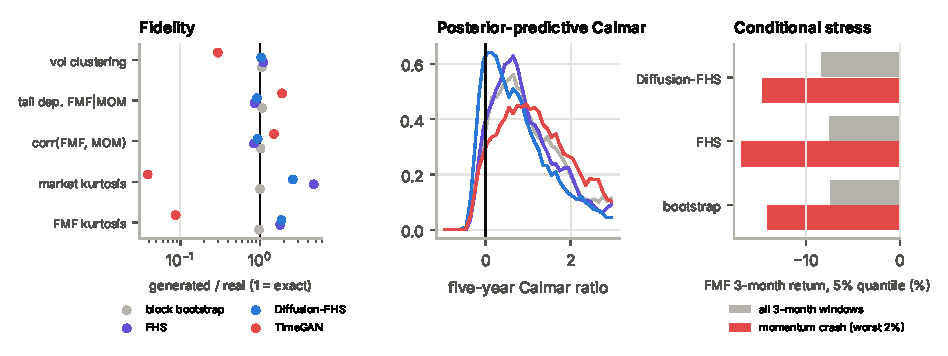
\includegraphics[width=\figw]{fig/fig18.pdf}
\caption{Left: stylised facts of real and generated data. Centre: distribution of the five-year Calmar ratio with posterior-predictive drift. Right: 5\% quantile of FMF-N's three-month return, unconditionally and in simulated momentum crashes.}\label{fig:generative}
\end{figure}
